\documentclass[11pt, a4paper, twoside]{Thesis}
\usepackage{etex}
%\usepackage{arabtex}
%\usepackage{utf8}

\usepackage{subcaption}
%\usepackage{amsmath}
\usepackage{tocbibind}
%\usepackage{packages/algorithm2e}
\usepackage{multirow}
\usepackage{setspace}
\usepackage{tikz}
\usetikzlibrary{shapes.geometric, arrows}
\usepackage{microtype}

\usepackage{standalone}
\usepackage{tabularx}

\newcolumntype{Y}{>{\centering\arraybackslash}X}

\setlength{\parindent}{0.7cm}

\makeatletter
\DeclareRobustCommand\onedot{\futurelet\@let@token\@onedot}
\def\@onedot{\ifx\@let@token.\else.\null\fi\xspace}



\def\eg{\emph{e.g}\onedot} \def\Eg{\emph{E.g}\onedot}
\def\ie{\emph{i.e}\onedot} \def\Ie{\emph{I.e}\onedot}
\def\cf{\emph{c.f}\onedot} \def\Cf{\emph{C.f}\onedot}
\def\etc{\emph{etc}\onedot} \def\vs{\emph{vs}\onedot}
\def\wrt{w.r.t\onedot} \def\dof{d.o.f\onedot}
\def\etal{\emph{et al}\onedot}
\usepackage[group-separator={,}]{siunitx}

\makeatother

\newcommand{\argmax}{\operatornamewithlimits{argmax}}
\newcommand{\argmin}{\operatornamewithlimits{argmin}}
\newcommand{\abs}[1]{\left\lvert#1\right\rvert}
\newcommand{\norm}[1]{\left\lVert#1\right\rVert}
\newcommand{\listofalgorithmes}{\tocfile{\listalgorithmcfname}{loa}}
\newcommand\Chapter[2]{
  \chapter[#1: {\itshape#2}]{#1\\[1ex]\Large#2}
}

\begin{document}
%\setcode{utf8}

% *************** Front matter ***************
\frontmatter

\title  {Towards Nonmonotonic Relational Learning from Knowledge Graphs}

\authors  {\texorpdfstring
            {{Hai Dang Tran}}
            {}
            }
\addresses  {\groupname\\\deptname\\\univname}  % Do not change this here, instead these must be set in the "Thesis.cls" file, please look through it instead
%\usdate
\date       {Saarbr\"ucken, \today }
\subject    {}
\keywords   {}

\maketitle

%\newpage
%\mbox{}
%\thispagestyle{empty}
%\newpage

\setstretch{1.3}

\thispagestyle{empty}

\section*{Eidesstattliche Erkl\"{a}rung}
Ich erkl\"{a}re hiermit an Eides Statt, dass ich die vorliegende Arbeit selbstst\"{a}ndig verfasst und keine
anderen als die angegebenen Quellen und Hilfsmittel verwendet habe.

\vspace{0.60cm}
\section*{Statement in Lieu of an Oath}
I hereby confirm that I have written this thesis on my own and that I have not used any other media or
materials than the ones referred to in this thesis.
\vspace{1.5cm}

\section*{Einverst\"{a}ndniserkl\"{a}rung}
Ich bin damit einverstanden, dass meine (bestandene) Arbeit in beiden Versionen in die Bibliothek der
Informatik aufgenommen und damit ver\"{o}ffentlicht wird.

\vspace{0.60cm}
\section*{Declaration of Consent}
I agree to make both versions of my thesis (with a passing grade) accessible to the public by having
them added to the library of the Computer Science Department.
\vspace{3cm}

\begin{flushright}
\noindent Saarbr\"{u}cken, \today
\hfill
Hai Dang Tran
\end{flushright}

\clearpage  % Declaration ended, now start a new page
%% ----------------------------------------------------------------

\newpage
\mbox{}
\thispagestyle{empty}
\newpage

% The Abstract Page
\addtotoc{Abstract}  % Add the "Abstract" page entry to the Contents
\abstract{
\addtocontents{toc}{\vspace{1em}}  % Add a gap in the Contents, for aesthetics

These days witness the development of information extraction, which leads to the birth of knowledge graphs (KGs), that is, large collections of relational facts. Though information extraction tools can be executed automatically, it is not guaranteed that the KGs they produce are complete. Hence, Open World Assumption (OWA) should be applied to these graphs, that is, facts which are not given can be treated as true or false. Rule mining approaches can be applied to tackle the problem of KG completion. Nonetheless, the existing approaches pay attention to positive rules, which do not take exceptions or negated atoms into consideration and may therefore infer wrong facts. Recently a rule-based technique that bridges this gap has been proposed, but it only works on flattened presentation of a KG, that is, a collection of unary facts. This work extends the previous results and presents an approach for mining exception enriched rules over KGs in their original relational form.

The contributions of this thesis are: (i) we introduce a framework to revise positive rules and improve quality of KGs, (ii) from given KG and a set of positive rules, we propose a method for finding exception candidates, assessing their quality and ranking them based on chosen measure with a novel concept of partial materialization, (iii) we implement a system and conduct experiments to test our methodology and they demonstrate promising results.
\begin{itemize}
\item need to add here
\end{itemize}
}
\clearpage

%% ----------------------------------------------------------------
\newpage
\mbox{}
\thispagestyle{empty}
\newpage

\setstretch{1.3}  % Reset the line-spacing to 1.3 for body text (if it has changed)

% The Acknowledgements page, for thanking everyone
\acknowledgements{
\addtocontents{toc}{}  % Add a gap in the Contents, for aesthetics    \vspace{1em}


}
\clearpage  % End of the Acknowledgements
%% ----------------------------------------------------------------
\newpage
\mbox{}
\thispagestyle{empty}
\newpage

\newpage
\mbox{}
\thispagestyle{empty}
\newpage

\setstretch{1}
\begin{spacing}{0.1}
\pagestyle{fancy}
\tableofcontents
\newpage
\listoffigures
\newpage
\listoftables
\newpage
%\listofalgorithmes
\end{spacing}

\clearpage

\setstretch{1.3}
% *************** Main matter ***************
\mainmatter

\chapter{Introduction}
\label{chap:intro}

\section{Motivation}
\label{chap:motivation}

These days witness the development of information extraction methods, which are fruitfully exploited for automatic construction of Knowledge Graphs (KGs). These are large collections of relational facts in the \textit{$\langle$subject predicate object$\rangle$} format. Such triples reflect facts about the real world, which can be converted to facts over unary and binary relations in predicate calculus. Every such triple can be represented as a binary fact \textit{predicate(subject, object)} if \textit{predicate} is not a \textit{type} and a unary fact \textit{object(subject)} otherwise. For example, \textit{$\langle$Brad livesIn Berlin$\rangle$} can be rewritten as $livesIn(Brad, Berlin)$ while \textit{$\langle$Mat type artist$\rangle$} can be converted to $artist(Mat)$. Examples of KGs include YAGO~\cite{ref28}, Wikidata~\footnote{\url{https://www.wikidata.org}}, Freebase~\footnote{\url{https://developers.google.com/freebase/}}, etc (see Chapter~\ref{chap:relwork} for details).

Unfortunately, KGs are normally incomplete due to their automatic construction. Hence, they are processed under the Open World Assumption (OWA) where missing facts can be true or false. Therefore, the \textit{knowledge completion problem} (also known as \textit{link prediction}) plays an important role in improving the quality of KGs. To achieve this, rule learning approaches~\cite{ref39, ref10} are used to create rules which can infer new potentially missing facts. However, the existing methods only pay attention to positive rules, which do not take exceptions (negated atoms) into consideration and may therefore make wrong predictions. For instance, a rule:

\begin{equation}
r1: livesIn(X,Z) \leftarrow isMarriedTo(X,Y), livesIn(Y,Z)
\end{equation}
\label{rule1}

\noindent can be discovered from the graph in Figure~\ref{fig1.1} and exploited to predict new facts $livesIn(Alice, Berlin), livesIn(Dave, Chicago)$ and $livesIn(Lucy, Amsterdam)$. However, in reality the first two facts might be incorrect, since $Alice$ and $Dave$ are researchers and the rule $r1$ might have researcher as an exception. Exceptions should be taken into account in rule learning to improve both the rule quality and the quality of facts it produces.

\begin{figure}[t]
\centering
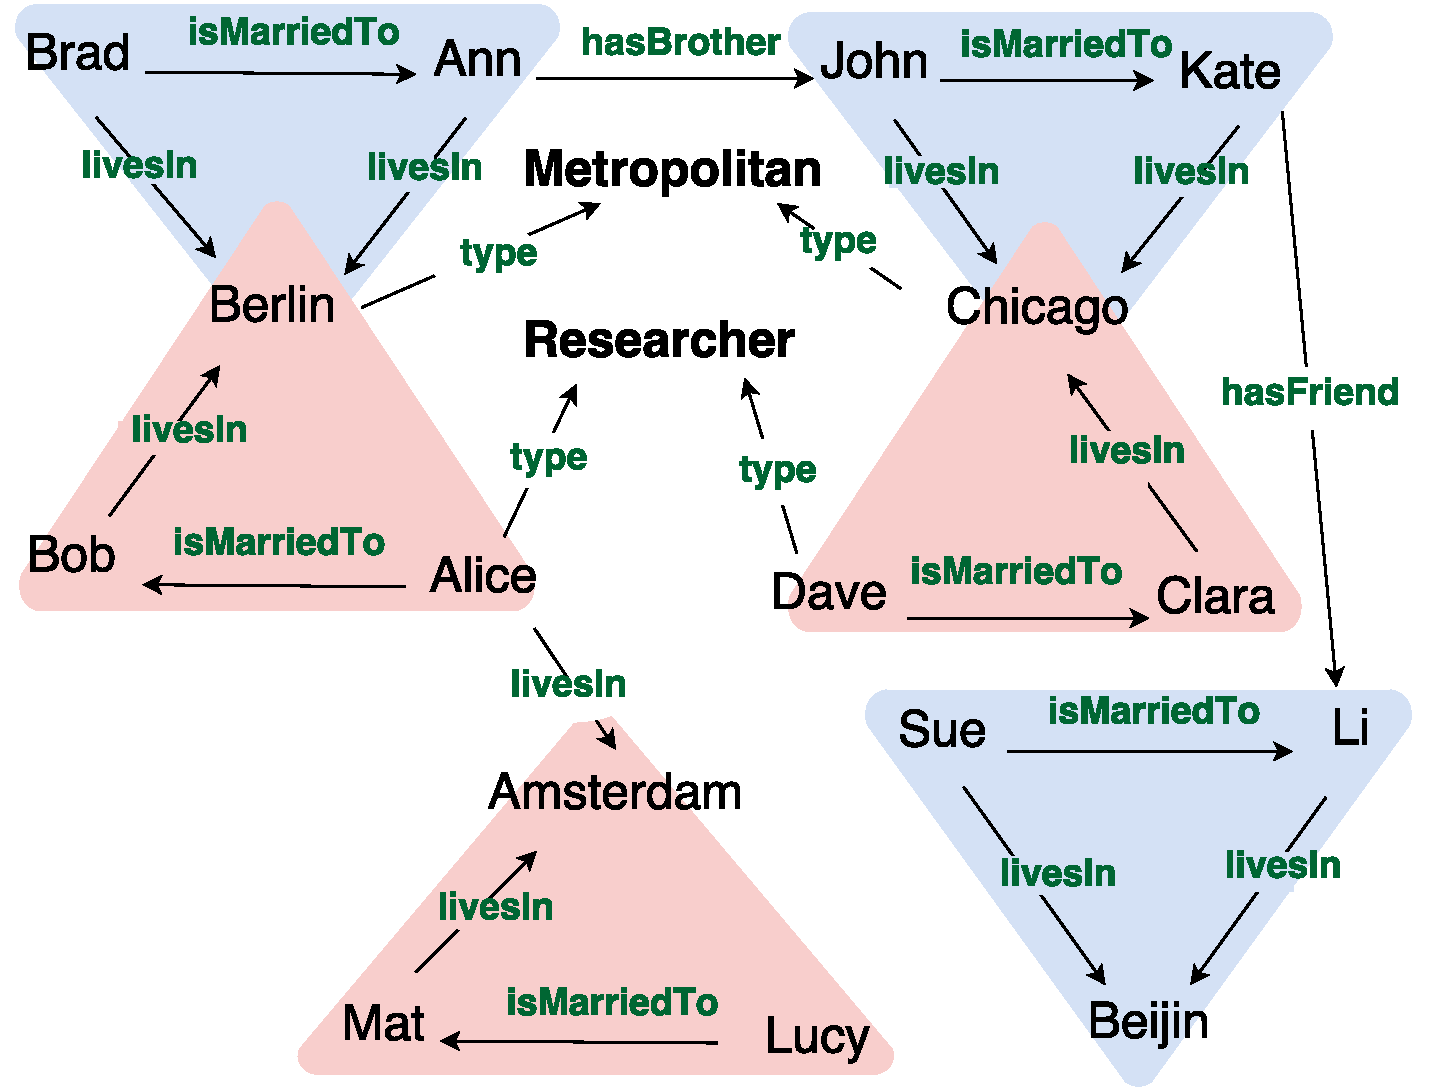
\includegraphics[width=0.75\textwidth]{figures/kg_advanced_col}
\caption{A Visualization of a Knowledge Graph}
\label{fig1.1}
\end{figure}

\section{State of the Art and Its Limitations}

\textit{Nonmonotonic rule learning}~\cite{ref11, ref40, ref41, ref32, ref42} focuses on discovering a set of rules with exceptions (negated atoms) in their bodies (see Chapter \ref{chap:back} for details). However, the state-of-the-art nonmonotonic ILP algorithms cannot be directly applied to our problem due to the following reasons:
\begin{itemize}
\item The \textit{target relations} cannot be explicitly defined because we do not know which parts of the graph need to be extended. A naive solution to this issue is to mine all possible rules for the available predicates in the KG. However, this solution is computationally expensive due to the large number of facts in the original KGs.
\item Second, ILP systems usually exploit positive and \textit{negative examples}. While positive examples are available in our work, negative ones are not given. Besides, the latter are difficult to collect because we cannot differentiate between wrong and unseen triples. Thus, a simple approach to overcome this is to discover rules from solely positive facts.
\item Finally, the \textit{language bias} is not easy to define since the schema of the original data is not given.
\end{itemize}

To overcome the above obstacles, casting our problem into an exploratory data analysis is a suitable solution. The authors in~\cite{ref12} propose association rule mining methods to explore positive (Horn) rules, and then revise them by inserting exceptions or negated atoms into their bodies to improve the predictive quality of the rules. However, this approach only works on a flattened presentation of a KG, i.e., a collection of unary facts.

\section{Goals}

The aim of this thesis is to:
\begin{itemize}
\item Propose a theory to explore interesting and informative nonmonotonic rules.
\item Build a scalable system in terms of run time to generate rules with exceptions from a large collections of facts.
\item Extensively evaluate the developed system by performing experiments on the real world KGs.
\end{itemize}

\section{Contributions}

This thesis is an extension of the work~\cite{ref12} to handle KGs in their original form. More specifically, we want to mine rules with exceptions from a set of relational facts in KGs treated under the OWA. We transform the knowledge completion problem into \textit{theory revision} task, where given a KG and a set of previously learned Horn rules, the goal is to revise Horn rules to nonmonotonic ones by introducing exceptions. The positive rules can be found by using off-the-shell tools for association rule learning. The revision should be done with the purpose of improving the quality of the revised rules compared to their original versions. To estimate the quality, we exploit the conviction measure~\cite{ref48}.

Our approach consists of four steps. First, for each positive rule, we try to find normal and abnormal sets, that is, set of instances that follow and do not follow given rule, respectively. Second, we mine exception witness sets, that is, sets of unary or binary predicates that can explain abnormal instances. For example, \textit{Researcher} is a possible exception for the rule $r1$ based on the KG in Figure~\ref{fig1.1}. Third, we add exceptions to the Horn rules in the form of a single negated atom and define a measure to assess the quality of the obtained revisions. Importantly, the interaction between revised rules is taken into consideration in our approach by a novel concept of \textit{partial materialization}. Finally, exceptions are ranked based on the proposed measures, and the best revision is selected as the final solution. The contributions of this thesis can be summarized as follows:

\begin{itemize}
\item We introduce a framework to revise positive rules and improve their quality by incorporating negated atoms into their bodies.
\item We propose a method for finding exception candidates, assessing their quality and ranking them based on the defined measures. With the novel concept of \textit{partial materialization}, the cross-talk between the rules is taken into account during the revision process.
\item We develop a system RUMIS that mines Horn rules from a KG and enriches them with exceptions.
\item We construct benchmarks and conduct experiments with YAGO3, IMDB and a fragment of Wikidata to test the above-mentioned methodology and the partial materialization concept.
\end{itemize}

\section{Structure}

The outline of this thesis is as follows. Chapter~\ref{chap:relwork} describes related work and presents the literature review. Chapter~\ref{chap:back} provides background and preliminaries for nonmonotonic logic programs and relational association rule learning. Chapter~\ref{chap:frame} presents the rule learning problem that we are tackling and describes our methodology. Chapter~\ref{chap:system} contains the system overview, implementation details and optimization strategies. Chapter~\ref{chap:eval} describes the benchmark construction process, experimental results, their analysis and interpretation. Finally, Chapter~\ref{chap:conclusion} concludes the thesis and outlines further directions.

\chapter{Related Work}

The area of relational learning on semantic web has recently attracted interest from many researchers. The approaches that aim at tackling this problem can be mainly classified into two groups: statistics-based and logic-based. In this chapter we review semantic web and the relevant works from these groups.

\section{Semantic Web}

The Semantic Web enables computers to interpret the meaning of the data all over the Internet. Alternatively, it can be defined as ``a web of data that can be processed directly and indirectly by machines" in~\cite{ref26}.

The World Wide Web Consortium (W3C) defines the semantic web and the Resource Description Framework (RDF) as a platform for Linked Data~\cite{ref26}. The W3C proposes other technologies such as SPARQL, OWL for data manipulation. Architecture of the W3C can be presented as a stack in Figure~\ref{fig1}~\footnote{\url{https://www.w3.org/DesignIssues/diagrams/sweb-stack/2006a.png}}.

\begin{figure}
\centering
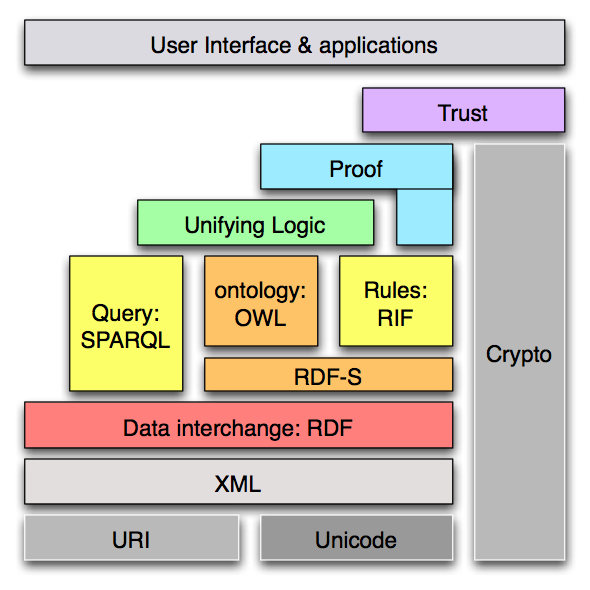
\includegraphics[width=0.65\textwidth]{semantic-web.png}
\caption{The Semantic Web technologies}
\label{fig1}
\end{figure}

The RDF can be used to describe knowledge graph where facts are presented in a format: \textit{$<$subject$>$ $<$predicate$>$ $<$object$>$}. This is the fundamental format of many knowledge bases such as YAGO~\cite{ref28}, FreeBase~\footnote{\url{https://developers.google.com/freebase/}}, Wikidata\footnote{\url{https://www.wikidata.org}}, etc. There are several typical knowledge graphs listed in Table~\ref{table1}~\cite{ref27} which have various scales. Of all the KB mentioned in the table, Google's Knowledge Graph is the largest with 18 billions facts. In our current work, we pay attention to YAGO, IMDB for experimental results.

Though having different number of predicates, entities and facts, these graphs share the following common properties~\cite{ref27}:

\begin{itemize}
\item Facts from real world are reflected in the knowledge graphs.
\item The domains are fruitful in the knowledge graphs, e.g., sports, arts, ...
\item The interconnection between knowledge graphs are taken into consideration, i.e., the mapping of entities and relations are explicitly indicated in each KB.
\end{itemize}

\begin{table}
\begin{center}
\begin{tabular}{|c|c|c|c|c|}
\hline
Name & Instances & Facts & Types & Relations\\
\hline\hline
DBpedia (English) & 4,806,150 & 176,043,129 & 735 & 2,813\\
\hline
YAGO & 4,595,906 & 25,946,870 & 488,469 & 77\\
\hline
Freebase & 49,947,845 & 3,041,722,635 & 26,507 & 37,781\\
\hline
Wikidata & 15,602,060 & 65,993,797 & 23,157 & 1,673\\
\hline
NELL & 2,006,896 & 432,845 & 285 & 425\\
\hline
OpenCyc & 118,499 & 2,413,894 & 45,153 & 18,526\\
\hline
Google's Knowledge Graph & 570,000,000 & 18,000,000,000 & 1,500 & 35,000\\
\hline
Google's Knowledge Vault & 45,000,000 & 271,000,000 & 1,100 & 4,469\\
\hline
Yahoo! Knowledge Graph & 3,443,743 & 1,391,054,990 & 250 & 800\\
\hline
IMDB & 117,551 & 134,639 & 17,049 & 39 \\
\hline
\end{tabular}
\end{center}
\caption{List of typical knowledge graphs}
\label{table1}
\end{table}

\section{Statistics-based Approaches}

The statistics-based approaches focus on building models with latent features which are not directly observable from the original data~\cite{ref1}. The core idea is to infer correlation between objects based on selected hidden features. Besides, feature extraction is automatically executed in these methods.

RESCAL is one of principal algorithms in this direction where relations of all hidden feature pairs are taken into consideration~\cite{ref2, ref3}. This method is extended to classical tensor decomposition algorithm~\cite{ref4} and neural tensor network~\cite{ref5}.

While many tensor factorization methods use subject, predicate and object as three dimensions to model a knowledge graph as a cube, some matrix decomposition algorithms try to transform this cube into two dimensional data. For instance, in~\cite{ref6, ref7} subject and object dimensions are merged into one representing a pair of entities.

Distance-based models use the intuition that entities have high chance to be related to each other if their hidden representation features are close to each other. The closeness can be checked based on some predefined distance measures. This approach can be expanded to structure embedding model~\cite{ref8}.

\section{Logic-based Approaches}

The logic-based approaches aim at finding observable patterns in order to infer new links in the knowledge graph~\cite{ref1}. Since the patterns can be directly seen in the data, these algorithms are more interpretable than the ones based on statistical approaches. For instance, a pattern extracted from the graph can be represented in the form:\\

\centerline{\textit{livesIn(Z, Y) $\leftarrow$ isMarriedTo(X, Z), livesIn(X, Y).}}

This form is equivalent to a triangle of three predicate edges in the knowledge graph. Since this pattern is frequent and observable, it can be mined in order to predict new links. More specifically, if we know some facts such as: \textit{isMarriedTo(Peter, Marry), livesIn(Marry, London)}; then the fact \textit{livesIn(Peter, London)} is likely to be true.

In the rest of this section, several main logic-based systems are discussed in details and illustrated with typical examples.

\subsection{Inductive Logic Programming Systems}

Inductive Logic Programming~\cite{ref9} (ILP) is a combination of Machine Learning and Logic Programming fields and it is used for generating hypothesis based on background knowledge and specific examples. These examples can be classified into positive and negative ones. The goal is to find a hypothesis that covers all positive examples and none of the negative ones.

Rule mining is a core problem in ILP, however, applying ILP algorithms to semantic web data is problematic for the following reasons. First, ILP tools are not scalable and efficient for large knowlege graphs such as YAGO, Freebase, Wikidata~\cite{ref10}. In some experiments conducted in~\cite{ref10}, it takes several days to process YAGO2 data using cutting edge ILP tools such as ALEPH~\cite{ref14, ref10}, QuickFoil~\cite{ref15, ref10}.

Second, ILP methods use closed world assumption (CWA), under which a given KB is assumed to be complete and missing facts are treated as false rather than unknown. These methods require both positive and negative examples like traditional machine learning algorithms. This assumption and requirement are not suitable for our problem since there are only in-completed positive facts in real world data~\cite{ref10}.

Third, most ILP algorithms generate positive Horn rules without exceptions~\cite{ref11}. Since these rules may have low precision, exceptions should be taken into consideration to improve quality of predicted facts. As a result, mining exceptions is an important purpose of our work and naively using ILP techniques are not always suitable for us.

\textbf{ALEPH.} This name stands for A Learning Engine for Proposing Hypotheses which is one of the typical systems in ILP. This tool is developed and extended from P-Progol~\footnote{\url{http://www.cs.ox.ac.uk/activities/machinelearning/Aleph/aleph}}. Like many other ILP systems, as input ALEPH receives the background knowledge and sets of positive, negative examples. After that, it generates a set of rules as an output. More specifically, the tool processes head predicates alternatively. Experiments in~\cite{ref10} show that run time for each head relation varies widely from several seconds to days. This indicates that ALEPH is not scalable for large datasets.

\textbf{QuickFOIL.} To address the scalability issues of ILP systems, the system QuickFOIL which is an optimized version of FOIL~\cite{ref36} has been developed. QuickFOIL produces Horn rules in an iterative fashion. Whenever a rule at a certain stage covers an example, the latter is removed from the set. Intuitively, the collection of found rules in each step can be used to summarize original knowledge base. QuickFOIL uses data refinement and pruning techniques to process large-scale input with millions of triples. This tool is a traditional ILP system since it requires negative examples and uses CWA assumption.

\subsection{Relational Learning Systems}

The systems in Relational Learning approaches do not require negative facts in the RDF data. Thus, the Open World Assumption (OWA) can be applied and this is one of pluses of these systems over ILP ones. In addition, with the aim to exploring more facts in KG, expanding by Relational Learning is more precise than traditional Information Extraction~\cite{ref29}. Indeed, publication~\cite{ref30} indicates that their authors use rule mining to generate more relations in YAGO2.

\textbf{WARMR.} The WARMR~\cite{ref16, ref17} system represents a combination of traditional ILP and rule learning approaches. Its algorithm performs level-wise searching and pruning to mine patterns~\cite{ref10}. To check the runtime performance of WARMR, AMIE+ authors~\cite{ref10} test it with YAGO2 dataset. The tool processes more than a day with YAGO2 and more than 15 hours with part of the dataset. It is also indicated in~\cite{ref10} that WARMR is developed with ProLog, and thus, is not fast to process big data.

\textbf{AMIE(+).} The scalability and CWA assumption issues of ILP are tackled in AMIE(+)~\cite{ref10} system. This tool receives a large knowledge graph as an input and generates top positive Horn rules with high quality. Initially, AMIE begins with a list of rules with empty body and binary head predicate. After that, the rules can be expanded with additional relations and variables by three mining operators~\cite{ref10}. These operators are executed by query manipulation to explore new predicates and instances. As regards the implementation, AMIE uses in-memory database with fact indexes to run select and existence queries~\cite{ref10}.

AMIE+ is a new version of AMIE in which run time performance is enhanced by pruning and optimizing evaluation. While the former is implemented by query refining, the latter uses measure approximation. Experimental work in~\cite{ref10} shows that this platform can process millions of triples in RDF graph and its mined rules surpass those of other methods in terms of efficiency.

\textbf{RDF2Rules.} The RDF2Rules~\cite{ref29} focuses on mining cycle patterns on KG, in the next step, rules are discovered based on these relation cycles. Besides, this tool takes care about type of entities for the Horn rules. Thanks to this, the rule quality is enhanced and the authors use a new confidence measure to check this instead of PCA measure~\cite{ref10} in AMIE paper. Experiments show that this tool is efficient, especially with rules containing entity type, it run much faster than AMIE+. However, the cycle form is a restricted condition and it is better if the publication expands this to many different relation patterns.

Like other ILP platforms, Relational Learning tools do not take care of nonmonotonic rules, i.e., rules with exceptions since its output is a list of Horn rules. Our work can solve this problem because it aims at generating nonmonotonic rules from a list of positive rules and a big knowledge graph.

\subsection{Nonmonotonic Rule Mining Systems}
\label{related-work-nonmonotonic-rule-mining-systems}

While traditional ILP systems do not take into account exceptions or negative atoms, the converse is true for Nonmonotonic Rule Mining systems. As regards a relation between ILP and Abductive Logic Programming (ALP~\cite{ref31}), some research works~\cite{ref11, ref32, ref33} are conducted to find rules with exceptions. However, CWA is used and all unseen triples are treated as false facts in these publications. This setting cannot be applied to our current work.

There are some nonmonotonic rule learning methods taking the uncompleted data into consideration in ~\cite{ref34}. This work pays attention to complicated association between different semantic parts. This is different from the current work where we focus on how good is new predicted data.

\textbf{Nonmonotonic Rule Mining with OWA and flattened data.} Research in~\cite{ref12} bases on OWA instead of CWA in some mentioned systems. This tool works on flattened knowledge graph, i.e., the graph that all RDF triples are converted to unary facts by concatenating predicates and objects. More specifically, a binary fact such as \textit{bornIn(s1, US)} can be transformed to unary form \textit{bornInUS(s1)}. Thanks to this, a knowledge graph can be converted to a binary transaction table as in Table~\ref{table2} where 1 or 0 mean the corresponding fact appear in the original graph or not. As a result, the authors in~\cite{ref12} may apply Item Set Mining algorithms~\cite{ref37} to find patterns. These patterns can be used to mine positive rules using Association Rule Mining tools~\cite{ref13}.

\begin{table}
\begin{center}
\begin{tabular}{|c|c|c|c|c|}
\hline
 & bornInUS & livesInUS & immigratesToUS & livesInUK\\
\hline\hline
s1 & 1 & 1 & 0 & 0\\
\hline
s2 & 1 & 0 & 1 & 1\\
\hline
s3 & 1 & 1 & 0 & 1\\
\hline
s4 & 0 & 0 & 1 & 0\\
\hline
s5 & 1 & 0 & 0 & 1\\
\hline
s6 & 0 & 0 & 1 & 1\\
\hline
s7 & 0 & 0 & 1 & 1\\
\hline
s8 & 1 & 0 & 0 & 0\\
\hline
s9 & 1 & 1 & 1 & 1\\
\hline
s10 & 0 & 1 & 0 & 1\\
\hline
\end{tabular}
\end{center}
\caption{Transaction table as flattened knowledge graph data.}
\label{table2}
\end{table}

In the next step, the exceptions for each rule are found based on normal and abnormal sets. Then these negative atoms are ranked based on several score measures and innovative concept of Partial Materialization (PM)~\cite{ref12}. In details, PM is the technique that some new predicted facts of other rules are used to measure the quality of a particular one. With the Ordered Partial Materialization (OPM), the idea is similar. The only difference is that the order of rules matters and new generated facts of previous rules instead of all other ones are counted for statistics.

From the same concept of Partial Materialization and above setting, we extend this work to the master thesis using different predictive measures. Another difference between the thesis and~\cite{ref12} is the format of the data. While la latter convert relations to unary forms, the former retains it in nature format. Thus, binary predicates with subjects and objects may appear in the resulting rules, not just the unary ones.

%\section{Other Approaches}
%
%Both of above-mentioned approaches are internal methods, that is, only data inside the graph is used to infer new relations. On the contrary, this section focuses on different approaches that require data outside the knowledge base, e.g., web pages linking to objects or big collection of documents.
%
%Wikipedia pages can be used to identify relations between entities in~\cite{ref18}. In a larger scale,~\cite{ref19} proposes learning lexical predicate patterns, and searches all over the Internet to find subject-object pairs corresponding to the patterns. These new pairs can be filled to the original graph. As a result, a big text corpora is used in ~\cite{ref19} to learn relations.
%
%With the intuition that entities appearing in the same table should have the same relations, authors in~\cite{ref20} try to refine knowledge graph based on Wikipedia tables. Similar research works are conducted using page lists~\cite{ref21} or HTML tables~\cite{ref22}.
%
%Instead of documents, interlinks are used to add relation edges to knowledge graph~\cite{ref23, ref24}. More specifically, relations of two entities in FreeBase can be inserted to YAGO if they also appear in the latter knowledge graph. This way can be extended to mapping method with probabilities in~\cite{ref25}.

\chapter{Background}
\label{chap:back}

In this chapter, we introduce some preliminary knowledge for the rest of the thesis with the following organization. First, nonmonotonic logic programs under answer set semantics and KG completion problem are presented. Second, we address some definitions of relational association rule mining such as \textit{head support, absolute support, confidence} and \textit{conviction}. These definitions are exploited in the main part of this work (Chapter~\ref{chap:frame} and~\ref{chap:system}).

\section{Nonmonotonic Logic Program}

In the current work, we rely on the standard definitions of logic programs~\cite{ref49}. Formally, \textit{nonmonotonic logic program P} is a rule set where each rule has the form:

\begin{equation}
r: H \leftarrow B, not E
\end{equation}
\label{rule3}

In details, $H$ stands for \textit{head(r)} which is a head of the rule $r$, i.e., a first-order atom in the format \textit{a(\textbf{X})}. Besides, \textit{B, not E} is a conjunction: \textit{b$_1$(\textbf{Y}$_1$), b$_2$(\textbf{Y}$_2$), ..., b$_k$(\textbf{Y}$_k$)} and \textit{not b$_{k+1}$(\textbf{Y}$_{k+1}$), not b$_{k+2}$(\textbf{Y}$_{k+2}$), ..., not b$_n$(\textbf{Y}$_n$)}, resp. $B$ and \textit{not E} are used as a short form of $body^+(r)$ and $body^-(r)$, resp. The $not$ operator is called the \textit{negation as failure (NAF) or default negation}. If $body^-(r) = \emptyset$ then $r$ is a positive (Horn) rule. \textit{\textbf{X, Y$_{1}$, Y$_{2}$, ..., Y$_{n}$}} are tuples of arguments, i.e., variables and/or constants and their sizes are the arity of \textit{a, b$_1$, b$_2$, ..., b$_n$}, resp. The signature of the program $P$ is denoted as $\Sigma_{P} = \langle$\textbf{P}$, \cC\rangle$ where \textbf{P}, $\cC$ are the sets of predicates and constants in $P$, resp.

A logic program $P$ is \textit{ground} if it does not contain any variables, i.e., only constants and predicates can appear in each rule $r$. For a non ground program $P$, $Gr(P)$ is a ground instantiation of $P$ which is obtained by replacing variables with constants in all possible ways. The \textit{Herbrand Universe HU(P)} of $P$ is the set of constants $\cC$ appearing in the program $P$ and \textit{Herbrand Base HB(P)} contains all possible ground atoms constructed by predicates in $P$ and constants in $\cC$, resp. Any subset of $HB(P)$ is a \textit{Herbrand Interpretation} of a program $P$. An interpretation $I$ is a model of a rule $r$ if for every possible substitution of variables with constants for which $body^+(r), body^-(r)$ are true, $head(r)$ is also true w.r.t. $I$. $I$ is defined as a model of a program $P$ if it satisfies all rules in $P$. In addition, $MM(P)$ denotes a set of a subset-inclusion minimal models of $P$.

An \textit{answer set} $I$ of $P$ is a Herbrand interpretation of $P$ s.t. $I \in MM(P^I)$. Here, $P^I$ denotes the Gelfond-Lifschitz (GL) reduct~\cite{ref50} of $P$ which is generated by deleting any rule $r$ s.t. $body^-(r)$ intersects with $I$ and then removing all NAFs in the rest of the rules. $AS(P)$ stands for the set of all answer sets for $P$.

\begin{example}\label{ex:as}
Consider the following nonmonotonic program as an example:\\
{\small \leftline{$P = \left\{
            \renewcommand{\arraystretch}{1.1}
            \begin{array}{@{\,}l@{~~}l@{}}
              \mbox{(1) }\mi{livesIn(brad,berlin)};\;\mbox{(2) }\mi{isMarriedTo(brad,ann)};\\
              \mbox{(3) } \mi{livesIn(Y,Z)\leftarrow isMarriedTo(X,Y),livesIn(X,Z),  \naf\ researcher(Y)}\\
            \end{array}%
            \!\right\}$}}

\normalsize
{\smallskip

\noindent            
We obtain the ground instantiation $Gr(P)$ of $P$ by replacing $X,Y,Z$ with $\mi{brad, \,ann}$ and $\mi{berlin}$, resp. Consider the interpretation $I=\{${\small\textit{isMarriedTo(brad,ann), livesIn(ann,berlin), livesIn(brad,berlin)}}$\}$. Based on the above definition, the GL-reduct $P^I$ of $P$ consists of a rule \textit{livesIn(ann,berlin) $\leftarrow$ livesIn(brad,berlin), isMarriedTo(brad,ann)} and the ground terms (1), (2). Since $I$ is a minimal model of $P^I$, by definition, we have that $I \in AS(P)$.}\qed
\end{example}

\section{Knowledge Graph Completion}

In this section, we provide a definition of a KG completion problem based on the above concept of Answer Set Programming. The factual representation of a KG $\cG$ is the set of ground atoms over the signature $\Sigma_{\cG}=\tuple{\mathbf{C},\mathbf{R},\mathcal{C}}$, in which $\mathbf{C}$, $\mathbf{R}$ and $\mathcal{C}$ denote the sets of unary predicates, binary predicates and constants, resp. By $\cG^i$, we denote a KG that contains all correct facts with predicates and constants from $\Sigma_{\cG^a}$ that are true in the real world. Based on~\cite{ref51}, the gap between the \emph{available graph} $\cG^a$ and $\cG^i$ is defined as follows.

\begin{definition}[Incomplete data source] A pair $G = (\cG^a, \cG^i)$ of two KGs is an incomplete data source, where $\cG^a\subseteq \cG^i$ and $\Sigma_{\cG^a}=\Sigma_{\cG^i}$.
\end{definition}

We aim at learning a nonmonotonic rule set $\cR$ from the $\cG^a$ s.t. application of $\cR$ to $\cG^a$ results in a good approximation of $\cG^i$. Application of $\cR$ to $\cG^a$ corresponds to the calculation of $I \in AS(\cR \cup \cG)$. More specifically, we define the rule based KG completion as follows:

\begin{definition}[Rule-based KG completion]\label{def:graphcompl}
Given a factual representation of a KG $\cG$ over the signature $\Sigma_{\cG}=\tuple{\mathbf{C},\mathbf{R},\cC}$ and a set of rules $\cR$ mined from $\cG$. The \emph{completion of $\cG$ \wrt\ $\cR$} is a graph $\cG_{\cR}$ constructed from any answer set in $AS(\cR \cup \cG)$.
\end{definition}

\section{Association Rule Mining in Relational Setting}

Association rule mining concerns the extraction of frequent patterns from the data and their subsequent casting into rules. Originally, association rules were studied in the market basket context, where interesting relations between products from transaction database of customer purchases were extracted, e.g., \textit{\{onions, potatoes\} $=>$ \{burger}\}~\cite{ref54}. Recently, association rule learning methods were extended to relational settings, which attracts research interests of both ILP~\cite{ref52} and KG~\cite{ref10} scientists. In the following description, we present typical rule measures for association rules in the relational setting.

A \emph{conjunctive query} $Q$ w.r.t $\cG$ is the expression of the form $Q(\vec{X}):-p_1(\vec{X_1}),\dotsc,p_m(\vec{X_m})$. The body (i.e., right part) of the query is a list of positive or negative atoms over $\cG$. The head (i.e., left part) is a tuple of variables appearing in the right part. The \emph{answer} of $Q$ w.r.t $\cG$ is defined as a set $Q(\cG):=\{$substitutions $\theta$ of $\vec{X}$: $p_i(\vec{X_i}\theta) \in \cG$ with $i \in [1..m]\}$. Based on \cite{ref53}, the \emph{(absolute) support} of a conjunctive query $Q$ w.r.t the KG $\cG$ is the cardinality of the set $Q(\cG)$. For instance, the query
\begin{equation}\mi{Q(X,Y,Z):-isMarriedTo(X,Y),\, }\mi{livesIn(Y,Z)}
\end{equation}
has the absolute support $6$ w.r.t $\cG$ in Figure~\ref{fig1.1} since there are $6$ substitutions for the triple $\langle X, Y, Z \rangle$ that satisfy \textit{isMarriedTo(X,Y), livesIn(Y,Z)} w.r.t $\cG$.

An \emph{association rule} is of the format $Q_1 => Q_2$, where $Q_1$ and $Q_2$ are conjunctive queries and all atoms in the body of $Q_1$ also appear in that of $Q_2$. For instance, from $Q(X,Y,Z)$ in the above example and
\begin{equation}Q'(X,Y,Z):-\mi{isMarriedTo(X,Y),\,livesIn(X,Z),\,} \mi{livesIn(Y,Z)}
\end{equation} the association rule $Q => Q'$ can be built.

In the current work, association rules are exploited with the aim to predict new facts, hence, they should be translated into logical format. More specifically, we convert the association rule $Q_1=>Q_2$ to the logical one $Q_2\backslash Q_1 \leftarrow Q_1$, where $Q_2 \backslash Q_1$ is the set of atoms which are in $Q_2$ but not in $Q_1$. For example, it can be seen that the above rule $Q=>Q'$ can be transformed to $\mi{r1}$ in Section~\ref{chap:intro}.

In this work, the conviction measure~\cite{ref48} is exploited for estimating the rule quality, since it is guaranteed to have high predictive power~\cite{ref46}. Hence, this measure is useful for KG completion introduced in Chapter~\ref{chap:frame}. With the rule $r:\;\mi{H\leftarrow B, \naf\ E}$, where $H=\mi{h(X,Y)}$ and $B,E$ contain a set of variables $\vec{Z}\supseteq X,Y$, we can find the \emph{conviction} by the following formula:
\vspace{-.26cm}
\begin{equation}
\mi{conv(r, \cG)= \dfrac{1 - supp(h(X,Y), \cG)}{1 - conf(r, \cG)}}
\end{equation}
in which $\mi{supp(h(X,Y),\cG)}$ stands for \textit{relative support} of the head $\mi{h(X,Y)}$, defined as:
\vspace{-.28cm}
\begin{equation}
supp(h(X,Y),\cG)=\dfrac{\#(X,Y):h(X,Y)\in \cG}{(\#X:\exists Y\;h(X,Y)\in \cG)*(\#Y:\exists X\;h(X,Y)\in \cG)}
\end{equation}
besides, $\mi{conf}$ denotes the \textit{confidence} of $r$:
\begin{equation}
conf(r,\cG)=\dfrac{\#(X,Y): H \in \cG, \exists \vec{Z}\;B\in \cG,E \not \in \cG}{\#(X,Y):\exists \vec{Z}\; B\in \cG, E \not \in \cG}
\end{equation}
\vspace{-.3cm}

\begin{example}
Applying these definitions to the KG in Figure~\ref{fig1.1}, we obtain the following results. Given a KG $\cG$ in Figure~\ref{fig1.1} and a rule $r1$ in the form~\ref{rule1}, there are three ways to substitute variables in $r1$ based on $\cG$. Thus, the absolute support of $r1$ w.r.t. $\cG$ is $3$. Besides, the \textit{relative head support} of predicates \textit{livesIn} and \textit{hasFriend} are $\mi{supp(livesIn(X,Z), \cG)}{=}\dfrac{9}{8 \times 4}{\approx} 0.3$ and  $\mi{supp(hasFriend(X,Z), \cG)}{=}\dfrac{1}{1 \times 1}{=} 1.0$, resp. The confidence of rule $r1$ is $conf(r1, \cG) {=} \dfrac{2}{5} {=} 0.4$, thus, the conviction measure is as follows $conv(r1, \cG) {=} \dfrac{1-0.3}{1 - 0.4} {=} \dfrac{7}{6} {=} 1.17$
\end{example}

% \begin{tabular}{|c|c|c|c|c|c|c|c|c|c|c|c|}
% \hline
%         \multirow{2}{*}{}              &   \multirow{2}{*}{Predicates}         & \multicolumn{3}{c|}{Predictions} & \multirow{2}{*}{Conflicts} & \multicolumn{2}{c|}{in $\cG_i$} & \multicolumn{2}{c|}{out $\cG_i$} & \multicolumn{2}{c|}{Removed Facts} \\ \cline{3-5} \cline{7-12} 
%                       &  & $\cR_\mi{H}$     & $\cR_{OPM}$     & $\cR_{\mi{OPM}}^{\mi{aux}}$     &    & $\cR_\mi{H}$     & $\cR_{\mi{OPM}}$ & $\cR_\mi{H}$     & $\cR_{\mi{OPM}}$            & Correctly    & Incorrectly   \\ \hline
% \multirow{5}{*}{YAGO} &     created       &        &     946     &              &    6                        &       &   29   &               &    917            &              &               \\ \cline{2-12}
%  &     dealsWith       &        &     4421     &              &    0                        &       &   52   &               &    4369            &              &               \\ \cline{2-12}
%  &     hasChild       &        &     2113     &              &    0                        &       &   143   &               &    1970            &              &               \\ \cline{2-12}
%  &     isCitizenOf       &        &     1146     &              &    5                        &       &   62   &               &    1084            &              &               \\ \cline{2-12}
%  &     livesIn       &        &     3746     &              &    5                        &       &   36   &               &    3710            &              &              
%   \\ \hline
% \multirow{7}{*}{IMDB} &     directed       &        &     339     &              &    0                        &       &   53   &               &    286            &              &               \\ \cline{2-12}
%   &     directedBy       &        &     429     &              &    0                        &       &   60   &               &    369            &              &               \\ \cline{2-12}
%  &     hasLanguage       &        &     248     &              &    0                        &       &   57   &               &    191            &              &               \\ \cline{2-12}
%    &     hasProductionLanguage       &        &     317     &              &    2                        &       &   149   &               &    168            &              &               \\ \cline{2-12}
%    &     producedIn       &        &     239     &              &    0                        &       &   54   &               &    185            &              &               \\ \cline{2-12}
%     &     writtenBy       &        &     5     &              &    0                        &       &   4   &               &    1            &              &               \\ \cline{2-12}
%     &     wrote       &        &     18     &              &    0                        &       &   7   &               &    11            &              &               \\ \cline{1-12}
% %%  \\ \hline
% \end{tabular}

\begin{tabular}{|c|c|c|c|c|c|c|c|c|c|c|c|c|c|}
\hline
 \multirow{2}{*}{}              &   \multirow{2}{*}{predicates}         & \multicolumn{3}{c|}{predictions} & \multicolumn{3}{c|}{conflicts}& \multicolumn{2}{c|}{in $\cG_i$} & \multicolumn{2}{c|}{outside $\cG_i$} & \multicolumn{2}{c|}{removed Facts} \\ \cline{3-14} 
         &  & $\cR_\mi{H}$     & $\cR_{OPM}$     & $\cR_{\mi{OPM}}^{\mi{aux}}$     & $\cR_{\mi{N}}$       & $\cR_{\mi{PM}}$     & $\cR_{\mi{OPM}}$  & $\cR_\mi{H}$     & $\cR_{\mi{OPM}}$ & $\cR_\mi{H}$     & $\cR_{\mi{OPM}}$            & Correctly    & Incorrectly   \\ \hline
\multirow{5}{*}{YAGO} &     dealsWith       &   4424     &     4423     &       188     & 0 &    0  &   0                   &      41 &   40   &      37582         &    36892            &              &               \\ \cline{2-14}
 &     hasChild       &    2134    &     2113     &      506        & 4 &           24      &  11       &   177    &   177   &    38390           &    37841            &              &               \\ \cline{2-14}
 &     influences       &  1045515      &     1041083     &     2696         &  0 &          993       &  1005      &    179   &   179   &       43880        &    41452            &              &               \\ \cline{2-14}
 &     isCitizenOf       &  28951      &     26930     &     65         & 0 &  0   &    0                  &   52    &   52   &     7665          &    7404            &              &               \\ \cline{2-14}
 &     participatedIn       &  134169      &     131711     &      511        &  14  &        14        &  14      &    314   &   314   &     35715          &    35206            &              &              
  \\ \hline
\multirow{3}{*}{IMDB} &     actedIn       &    1231    &    1214      &   28    &   194    &    104   &   194                  &    810   &   626   &    184424           &    168079            &              &               \\ \cline{2-14}
  &     hasGenre       &    1263    &     1230     &      17        & 5 &          4        &    5    &   106    &   105   &   7070            &    6370            &              &               \\ \cline{2-14}
 &     hasProductionLanguage       &   324     &     317     &      12        & 0  &         0        &   0     &   64    &   63   &  5260             &    5055            &              &               \\ \cline{1-14}
%%  \\ \hline
\end{tabular}

% \begin{tabular}{|c|c|c|c|c|c|c|c|c|c|c|c|c|c|}
% \hline
%  \multirow{2}{*}{}              &   \multirow{2}{*}{predicates}         & \multicolumn{3}{c|}{predictions} & \multicolumn{3}{c|}{conflicts}& \multicolumn{2}{c|}{in $\cG_i$} & \multicolumn{2}{c|}{outside $\cG_i$} & \multicolumn{2}{c|}{removed Facts} \\ \cline{3-14} 
%          &  & $\cR_\mi{H}$     & $\cR_{OPM}$     & $\cR_{\mi{OPM}}^{\mi{aux}}$     & $\cR_{\mi{N}}$       & $\cR_{\mi{PM}}$     & $\cR_{\mi{OPM}}$  & $\cR_\mi{H}$     & $\cR_{\mi{OPM}}$ & $\cR_\mi{H}$     & $\cR_{\mi{OPM}}$            & Correctly    & Incorrectly   \\ \hline
% \multirow{5}{*}{YAGO manual} &     actedIn       &   37623     &     36932     &       188     & 0 &    0  &   0                   &      41 &   40   &      37582         &    36892            &              &               \\ \cline{2-14}
%  &     diedIn       &    38567    &     38018     &      506        & 4 &           24      &  11       &   177    &   177   &    38390           &    37841            &              &               \\ \cline{2-14}
%  &     isCitizenOf       &  44059      &     41631     &     2696         &  0 &          993       &  1005      &    179   &   179   &       43880        &    41452            &              &               \\ \cline{2-14}
%  &     livesIn       &  7717      &     7456     &     65         & 0 &  0   &    0                  &   52    &   52   &     7665          &    7404            &              &               \\ \cline{2-14}
%  &     wasBornIn       &  36029      &     35520     &      511        &  14  &        14        &  14      &    314   &   314   &     35715          &    35206            &              &              
%   \\ \hline
% \multirow{6}{*}{IMDB top rules} &     actedIn       &    185234    &    168705      &   28    &   194    &    104   &   194                  &    810   &   626   &    184424           &    168079            &              &               \\ \cline{2-14}
%   &     directed       &    7176    &     6475     &      17        & 5 &          4        &    5    &   106    &   105   &   7070            &    6370            &              &               \\ \cline{2-14}
%  &     directedBy       &   5324     &     5118     &      12        & 0  &         0        &   0     &   64    &   63   &  5260             &    5055            &              &               \\ \cline{2-14}
%    &     hasGenre       &    38632    &     36794     &   25    &  19     &   11     &    19                &   1051    &   966   &       37581        &    35828            &              &               \\ \cline{2-14}
%    &     hasProdLang       &  8150      &     7995     &   8           & 0  &    3          &    3       &   1431    &   1403   &       6719        &    6592            &              &               \\ \cline{2-14}
%     &     hasSuccessor       &    261180    &     221145     &   34854           &  0  &      0      &  0          &    70   &   68   &      261110         &    221077            &              &               \\ \cline{1-14}
% %%  \\ \hline
% \end{tabular}

\chapter{Evaluation}
\label{chap:eval}

In this chapter, we present the evaluation results of the RUMIS system. We focus on testing the quality of rule revisions in terms of the conviction measure, as well the prediction quality. The chapter is organized as follows. First, the setting of the experiment is discussed. Second, the quality of rulesets and the facts they predict are assessed. Finally, we present the runtime performance of the system RUMIS on different real-world datasets.

\section{Setting}

\textbf{Dataset.} To measure the quality of rules and their predictions, the ideal graph $\cG^i$, i.e. the KG containing all true facts about the real world, is required. However, constructing $\cG^i$ is obviously not possible. Hence, instead we treat the given graph as an approximation of the ideal KG $\cG^i_{\mi{appr}}$. To obtain the available (training) KG $\cG^a$ we remove from $\cG^i_{\mi{appr}}$ 20\% of the facts for every binary relation, and retain all unary facts in $\cG^i_{\mi{appr}}$. It is guaranteed that there is no isolated vertex in $\cG^a$, i.e the node which is not connected to any other nodes in the graph. In our experiment, YAGO3~\cite{ref28}, Wikidata Football and IMDB~\footnote{\url{http://people.mpi-inf.mpg.de/~gadelrab/downloads/ILP2016}} datasets are used as the ideal KGs. YAGO3 covers a variety of domains and contains roughly 1.8 million entities, 38 predicates, and 20.7 million triples. Meanwhile, IMDB only focus on movie content collected from the IMDB website~\footnote{\url{http://imdb.com}}, there are 112 thousand entities, 38 predicates and 583 thousand triples in this KG. Besides, to construct the Wikidata Football for our experiments, we sample 1 million facts with 238 thousand entities and 443 predicates from football domain of the original Wikidata KG~\footnote{\url{https://www.wikidata.org}}. %In details, thanks to randomly choosing facts in the format \textit{$<$subject$>$ $<$memberOf$>$ $<$object$>$} where \textit{$<$object$>$} is in the list of manually chosen popular football clubs, famous footballers and coaches (seeding set) are sampled from Wikidata. After that, all the entities that can be visited from any node in the seeding set (chosen entities) by following paths (one or more consecutive links/edges/predicates in the original Wikidata KG) are collected for the ideal KG. These chosen entities and all possible links between them in the original Wikidata KG are sampled for the smaller scale. This new KG is expected to have specific domain where facts are related to football and sports.

Figure~\ref{fig:venn} depicts the ideal, approximated and available KGs as well the extended KGs $\cG_{\cR_{\mi{H}}}$, $\cG_{\cR_{\mi{NM}}}$ obtained by resp. applying $\cR_H$ and its revision $\cR_{NM}$ to $\cG^a$. The RUMIS system aims to tackle the KG completion problem by narrowing the difference between the $\cG_{\cR_{\mi{NM}}}$ and $ \cG^i$.

\begin{figure}[ht]
\centering
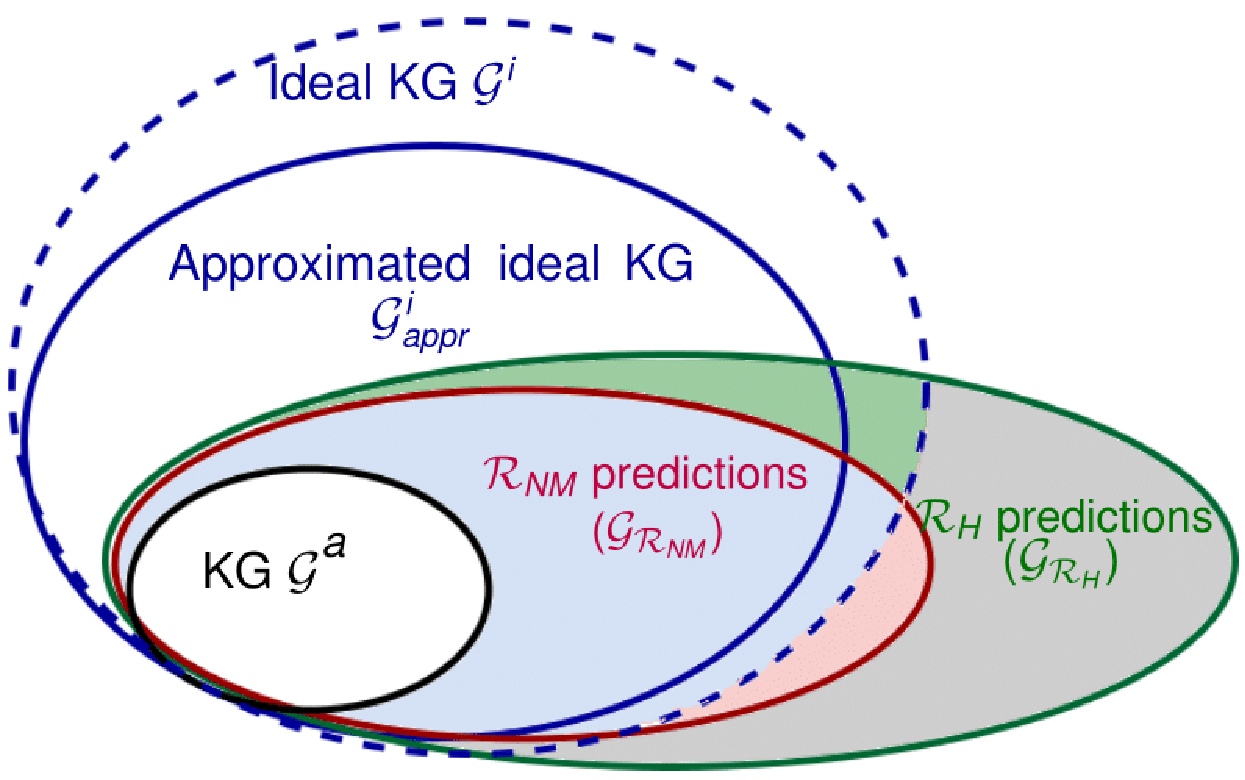
\includegraphics[width=0.55\textwidth]{figures/big_pic_exp}
\caption{The Ideal, Available and Extended KGs.}
\label{fig:venn}
\end{figure}

\textbf{Experimental Setup.} In our experiments, RUMIS is executed on a server which has Linux OS, 40 cores and 400GB RAM memory. As the data preparation, positive rules in the format \textit{h(X, Z) $\leftarrow$ p(X, Y), q(Y, Z)} are extracted from $\cG^a$ and ranked according to the \textit{absolute support} measure. The positive rule mining function of RUMIS (see Chapter~\ref{chap:system}) is exploited in this step. After that, the positive rules are revised following the approach presented in Chapter~\ref{chap:frame}. The \textit{conviction} measure is used as the $\mi{rm}$ rule measure. Various exception ranking earlier described strategies are realized in RUMIS. The resulting rule revisions are stored in $\mi{\cR_{N}}$, $\mi{\cR_{PM}}$, and $\mi{\cR_{OPM}}$, resp.

\section{Ruleset Quality}

We present the evaluation results of the rule quality assessment in Table~\ref{tab:rules_quality1} and~\ref{tab:rules_quality2} for YAGO, IMDB and Wikidata Football, resp. For every row in the tables, we fix the top-$\mi{k}$ ($k=5,30,$ ... $100$) positive rules $\cR_{H}$ that will be subsequently revised. Then the \textit{average conviction} of the rules and their revisions are found for YAGO, IMDB and Wikidata Football by using RUMIS. Naturally the quality of the revised rules is better than that of their positive versions w.r.t. conviction. Besides, in general while the average quality of every column has a decreasing trend with the appearance of rules having lower precision levels, the enhancement ratio between positive rules and their revisions increases and reaches the peak of $7.8\%$ and $10.3\%$ for top-100 IMDB and top-30 Wikidata Football rules, resp. The results show that the introduction of negated atoms significantly boost up the rule precision.

\begin{table}[ht]
\centering
\footnotesize
\renewcommand*{\arraystretch}{1.07}
\centering



%\footnotesize{
%\resizebox{\columnwidth}{!}{%
%
%\begin{tabular}{|l|llll|llll|llll|}
%\hline
%       \multirow{2}{*}{\textbf{\textit{topk}}}                    & \multicolumn{4}{c|}{\textbf{YAGO}}        & \multicolumn{4}{c|}{\textbf{IMDB}}  & \multicolumn{4}{c|}{\textbf{Sample WIKIDATA}}      \\ \cline{2-13} 
%       %\hline
% & $\cR_{H}$ & $\cR_{N}$ & $\cR_{PM}$ & $\cR_{OPM}$ & $\cR_{H}$ & $\cR_{N}$ & $\cR_{PM}$ & $\cR_{OPM}$ & $\cR_{H}$ & $\cR_{N}$ & $\cR_{PM}$ & $\cR_{OPM}$ \\ \hline
%5   & 1.3784 & 1.3821 & 1.3821 & 1.3821 & 2.2670 & 2.3014 & 2.3008 & 2.3014 & 3.2282 & 3.2342 & 3.2340 & 3.2342\\ %\hline
%30   & 1.1207 & 1.1253 & 1.1236 & 1.1237 & 1.5453 & 1.5644 & 1.5543 & 1.5640 & 3.1118 & 3.4315 & 3.4194 & \textbf{3.4271}\\ %\hline
%50   & 1.0884 & 1.0923 & 1.0909 & 1.0913 & 1.3571 & 1.3749 & 1.3666 & 1.3746  & 2.7115 & 2.9193 & 2.9070 & 2.9135\\ %\hline
%60   & 1.0797 & 1.0837 & 1.0823 & 1.0829 & 1.3063 & 1.3221 & 1.3143 & 1.3219  & 2.4930 & 2.7101 & 2.6986 & 2.7046\\ %\hline
%70   & 1.0714 & 1.0755 & 1.0736 & 1.0744 & 1.2675 & 1.2817 & 1.2746 & 1.2814  & 2.3395 & 2.5272 & 2.3931 & 2.5219\\ %\hline
%80   & 1.0685 & 1.0731 & 1.0710 & 1.0720 & 1.2368 & 1.2499 & 1.2431 & 1.2497  & 2.4071 & 2.5781 & 2.4597 & 2.5734\\ %\hline
%100   & 1.0618 & 1.0668 & 1.0648 & 1.0659 & 1.3074 & 1.4100 & 1.3987 & 1.4098  & 2.3258 & 2.4847 & 2.3859 & 2.4806\\ \hline
%
%\end{tabular}
%
%}
%}

\begin{tabular}{|l|llll|llll|}
\hline
       \multirow{2}{*}{\textbf{\textit{topk}}}                    & \multicolumn{4}{c|}{\textbf{YAGO}}        & \multicolumn{4}{c|}{\textbf{IMDB}}      \\ \cline{2-9} 
       %\hline
 & $\cR_{H}$ & $\cR_{N}$ & $\cR_{PM}$ & $\cR_{OPM}$ & $\cR_{H}$ & $\cR_{N}$ & $\cR_{PM}$ & $\cR_{OPM}$ \\ \hline
5   & 1.3784 & 1.3821 & 1.3821 & 1.3821 & 2.2670 & 2.3014 & 2.3008 & 2.3014\\ %\hline
30   & 1.1207 & 1.1253 & 1.1236 & 1.1237 & 1.5453 & 1.5644 & 1.5543 & 1.5640\\ %\hline
50   & 1.0884 & 1.0923 & 1.0909 & 1.0913 & 1.3571 & 1.3749 & 1.3666 & 1.3746\\ %\hline
60   & 1.0797 & 1.0837 & 1.0823 & 1.0829 & 1.3063 & 1.3221 & 1.3143 & 1.3219\\ %\hline
70   & 1.0714 & 1.0755 & 1.0736 & 1.0744 & 1.2675 & 1.2817 & 1.2746 & 1.2814\\ %\hline
80   & 1.0685 & 1.0731 & 1.0710 & 1.0720 & 1.2368 & 1.2499 & 1.2431 & 1.2497\\ %\hline
100   & 1.0618 & 1.0668 & 1.0648 & 1.0659 & 1.3074 & 1.4100 & 1.3987 & 1.4098\\ \hline

\end{tabular}

% \centering
% \caption{My caption}
% \label{my-label}
% \begin{tabular}{l|l|l|l|l|l|l|l|l|}
% \cline{2-9}
%                            & \multicolumn{4}{c|}{YAGO manual}        & \multicolumn{4}{c|}{IMDB top rules}        \\ \hline
% \multicolumn{1}{|l|}{\textit{topk}} & $\cR_{H}$ & $\cR_{N}$ & $\cR_{PM}$ & $\cR_{OPM}$ & $\cR_{H}$ & $\cR_{N}$ & $\cR_{PM}$ & $\cR_{OPM}$ \\ \hline
% \multicolumn{1}{|l|}{5}    &   1.10    &   1.11    &    1.20    &    1.15     &   2.27    &   2.3    &   2.89     &  2.55       \\ \hline
% \multicolumn{1}{|l|}{10}   &    1.10   &   1.11    &    1.23    &    1.18     &   1.9    &   1.92    &    4.74    &  2.07       \\ \hline
% \multicolumn{1}{|l|}{15}   &   1.12    &   1.13    &    1.32    &    1.18     &   1.8    &   1.82    &   5.25     &   1.98      \\ \hline
% \multicolumn{1}{|l|}{20}   &       &       &        &         &       &       &        &         \\ \hline
% \end{tabular}

\smallskip
\caption{The Average Quality of the Top Positive and Nonmonotonic Rules for YAGO, IMDB.}
\label{tab:rules_quality1}
%\vspace*{-1.7\baselineskip}
\end{table}

\begin{table}[ht]
\centering
\footnotesize
\renewcommand*{\arraystretch}{1.07}
\centering



%\footnotesize{
%\resizebox{\columnwidth}{!}{%
%
%\begin{tabular}{|l|llll|llll|llll|}
%\hline
%       \multirow{2}{*}{\textbf{\textit{topk}}}                    & \multicolumn{4}{c|}{\textbf{YAGO}}        & \multicolumn{4}{c|}{\textbf{IMDB}}  & \multicolumn{4}{c|}{\textbf{Sample WIKIDATA}}      \\ \cline{2-13} 
%       %\hline
% & $\cR_{H}$ & $\cR_{N}$ & $\cR_{PM}$ & $\cR_{OPM}$ & $\cR_{H}$ & $\cR_{N}$ & $\cR_{PM}$ & $\cR_{OPM}$ & $\cR_{H}$ & $\cR_{N}$ & $\cR_{PM}$ & $\cR_{OPM}$ \\ \hline
%5   & 1.3784 & 1.3821 & 1.3821 & 1.3821 & 2.2670 & 2.3014 & 2.3008 & 2.3014 & 3.2282 & 3.2342 & 3.2340 & 3.2342\\ %\hline
%30   & 1.1207 & 1.1253 & 1.1236 & 1.1237 & 1.5453 & 1.5644 & 1.5543 & 1.5640 & 3.1118 & 3.4315 & 3.4194 & \textbf{3.4271}\\ %\hline
%50   & 1.0884 & 1.0923 & 1.0909 & 1.0913 & 1.3571 & 1.3749 & 1.3666 & 1.3746  & 2.7115 & 2.9193 & 2.9070 & 2.9135\\ %\hline
%60   & 1.0797 & 1.0837 & 1.0823 & 1.0829 & 1.3063 & 1.3221 & 1.3143 & 1.3219  & 2.4930 & 2.7101 & 2.6986 & 2.7046\\ %\hline
%70   & 1.0714 & 1.0755 & 1.0736 & 1.0744 & 1.2675 & 1.2817 & 1.2746 & 1.2814  & 2.3395 & 2.5272 & 2.3931 & 2.5219\\ %\hline
%80   & 1.0685 & 1.0731 & 1.0710 & 1.0720 & 1.2368 & 1.2499 & 1.2431 & 1.2497  & 2.4071 & 2.5781 & 2.4597 & 2.5734\\ %\hline
%100   & 1.0618 & 1.0668 & 1.0648 & 1.0659 & 1.3074 & 1.4100 & 1.3987 & 1.4098  & 2.3258 & 2.4847 & 2.3859 & 2.4806\\ \hline
%
%\end{tabular}
%
%}
%}

\begin{tabular}{|l|llll|}
\hline
       \multirow{2}{*}{\textbf{\textit{topk}}}          & \multicolumn{4}{c|}{\textbf{WIKIDATA Football}}      \\ \cline{2-5} 
       %\hline
 & $\cR_{H}$ & $\cR_{N}$ & $\cR_{PM}$ & $\cR_{OPM}$ \\ \hline
5  & 3.2282 & 3.2342 & 3.2340 & 3.2342\\ %\hline
30   & 3.1118 & 3.4315 & 3.4194 & \textbf{3.4271}\\ %\hline
50   & 2.7115 & 2.9193 & 2.9070 & 2.9135\\ %\hline
60   & 2.4930 & 2.7101 & 2.6986 & 2.7046\\ %\hline
70   & 2.3395 & 2.5272 & 2.3931 & 2.5219\\ %\hline
80   & 2.4071 & 2.5781 & 2.4597 & 2.5734\\ %\hline
100   & 2.3258 & 2.4847 & 2.3859 & 2.4806\\ \hline

\end{tabular}

% \centering
% \caption{My caption}
% \label{my-label}
% \begin{tabular}{l|l|l|l|l|l|l|l|l|}
% \cline{2-9}
%                            & \multicolumn{4}{c|}{YAGO manual}        & \multicolumn{4}{c|}{IMDB top rules}        \\ \hline
% \multicolumn{1}{|l|}{\textit{topk}} & $\cR_{H}$ & $\cR_{N}$ & $\cR_{PM}$ & $\cR_{OPM}$ & $\cR_{H}$ & $\cR_{N}$ & $\cR_{PM}$ & $\cR_{OPM}$ \\ \hline
% \multicolumn{1}{|l|}{5}    &   1.10    &   1.11    &    1.20    &    1.15     &   2.27    &   2.3    &   2.89     &  2.55       \\ \hline
% \multicolumn{1}{|l|}{10}   &    1.10   &   1.11    &    1.23    &    1.18     &   1.9    &   1.92    &    4.74    &  2.07       \\ \hline
% \multicolumn{1}{|l|}{15}   &   1.12    &   1.13    &    1.32    &    1.18     &   1.8    &   1.82    &   5.25     &   1.98      \\ \hline
% \multicolumn{1}{|l|}{20}   &       &       &        &         &       &       &        &         \\ \hline
% \end{tabular}

\smallskip
\caption{The Average Quality of the Top Positive and Nonmonotonic Rules for Wikidata Football.}
\label{tab:rules_quality2}
%\vspace*{-1.7\baselineskip}
\end{table}

The enhancement ratio between revisions of the three ranking methods and the top positive rules is shown in Figure~\ref{fig_1_5_imdb}, ~\ref{fig_1_5_yago} and ~\ref{fig_1_5_wikidata} for IMDB, YAGO and Wikidata Football, resp. In these figures, the height and the width are corresponding to the top-$k$ and the improvement rate of the average conviction. One can observe that the rate has an uptrend, in general the more low quality Horn rules are added to the top ruleset, the higher is the improvement rate. The Naive ranking shows the best results w.r.t. the rule quality, which is obviously expected.

With IMDB dataset, the results of Naive and OPM ranking are approximately the same and slightly better than PM ranking. For the top-100 rules, the best average improvement of 7.8\% is achieved. It can be seen that the quality of positive rules around top-100 are much worse than the rest, resulting in the sharp increase between top-80 and top-100 in the Figure~\ref{fig_1_5_imdb}.

\begin{figure}[ht]
\centering
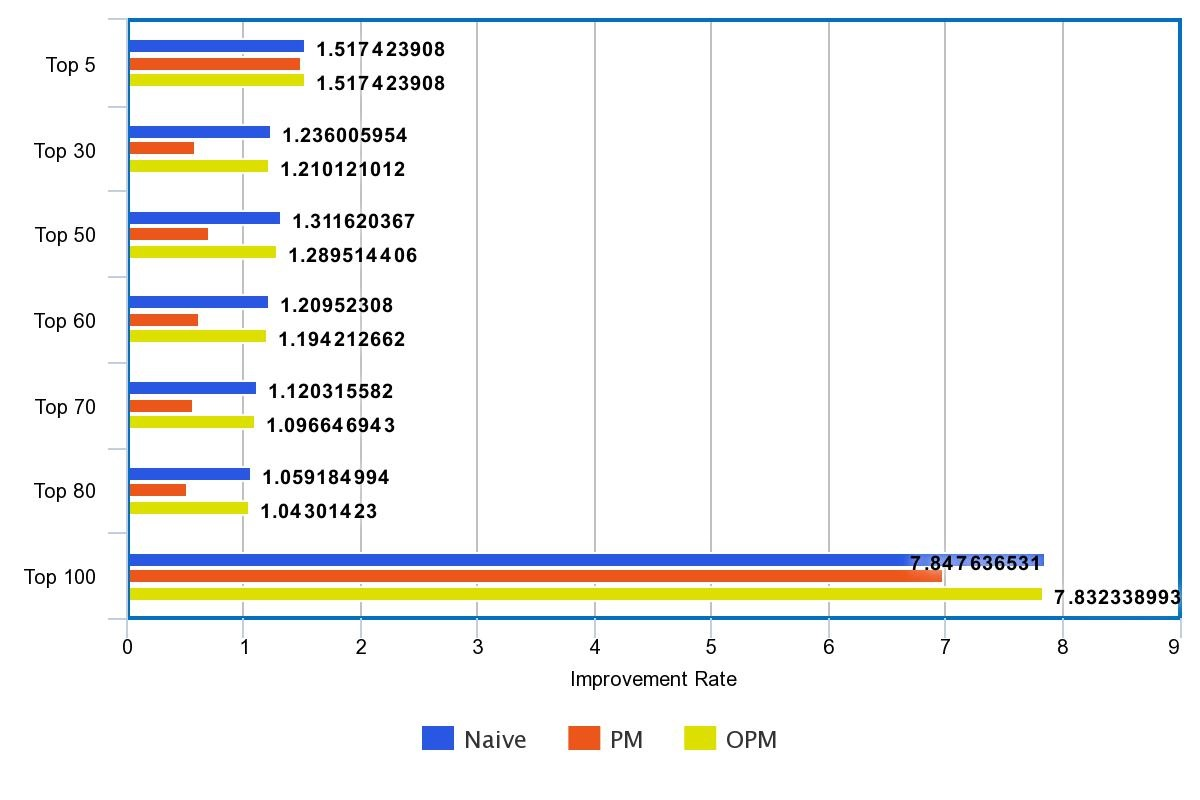
\includegraphics[width=0.85\textwidth]{figures/table_1_5_imdb.jpeg}
\caption{The Average Conviction Improvement Rate (\%) of Rules Revised using Our Methods and IMDB Dataset.}
\label{fig_1_5_imdb}
\end{figure}

In general, the improvement rates for the average conviction in YAGO increase. However, the contrast between the highest and the lowest in this figure is not as large as in IMDB data due to the qualities of top-100 Horn rules in YAGO are not highly different.

\begin{figure}[ht]
\centering
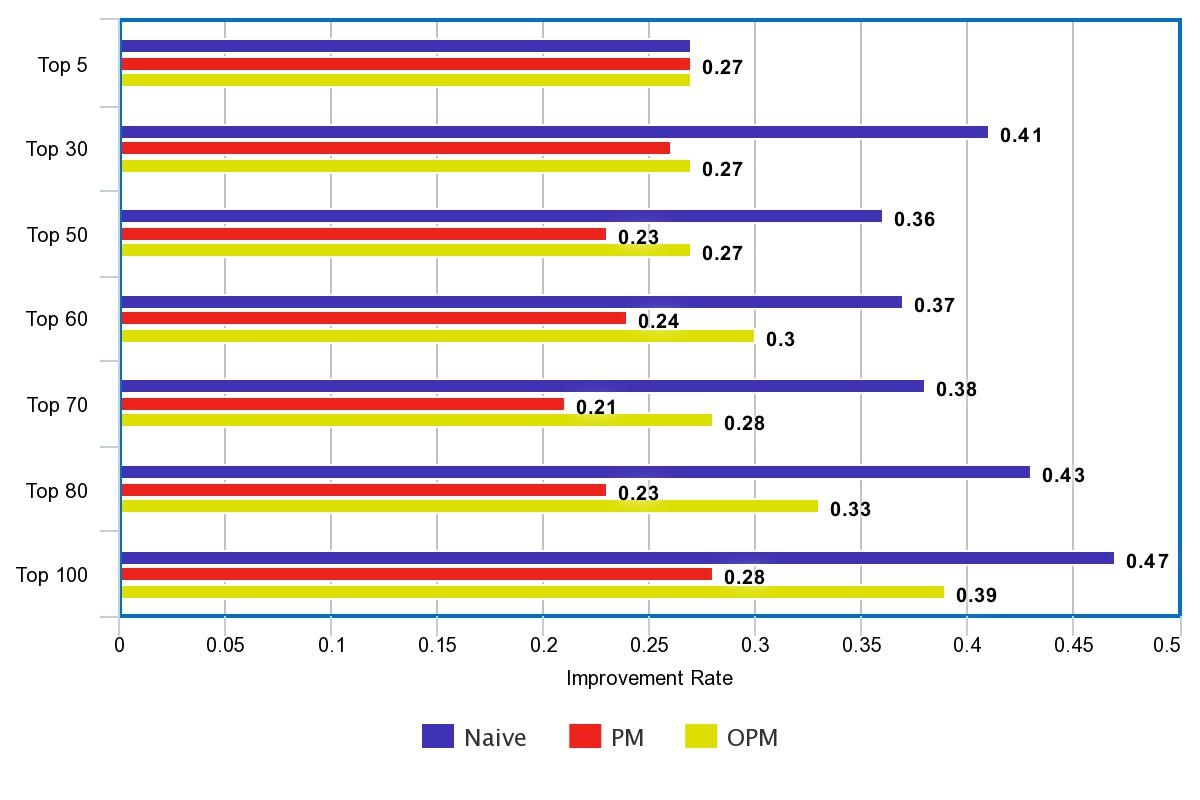
\includegraphics[width=0.85\textwidth]{figures/table_1_5_yago.jpeg}
\caption{The Average Conviction Improvement Rate (\%) of Rules Revised using Our Methods and YAGO Dataset.}
\label{fig_1_5_yago}
\end{figure}

As regards the Wikidata Football, Figure~\ref{fig_1_5_wikidata} witnesses an interesting pattern where the improvement rate significantly climbs from top-5 to top-30. It can be seen that RUMIS mines very good exceptions for positive rules around top-30, 
resulting in a peak of more than 10\% enhancement ratio for this dataset.

\begin{figure}[ht]
\centering
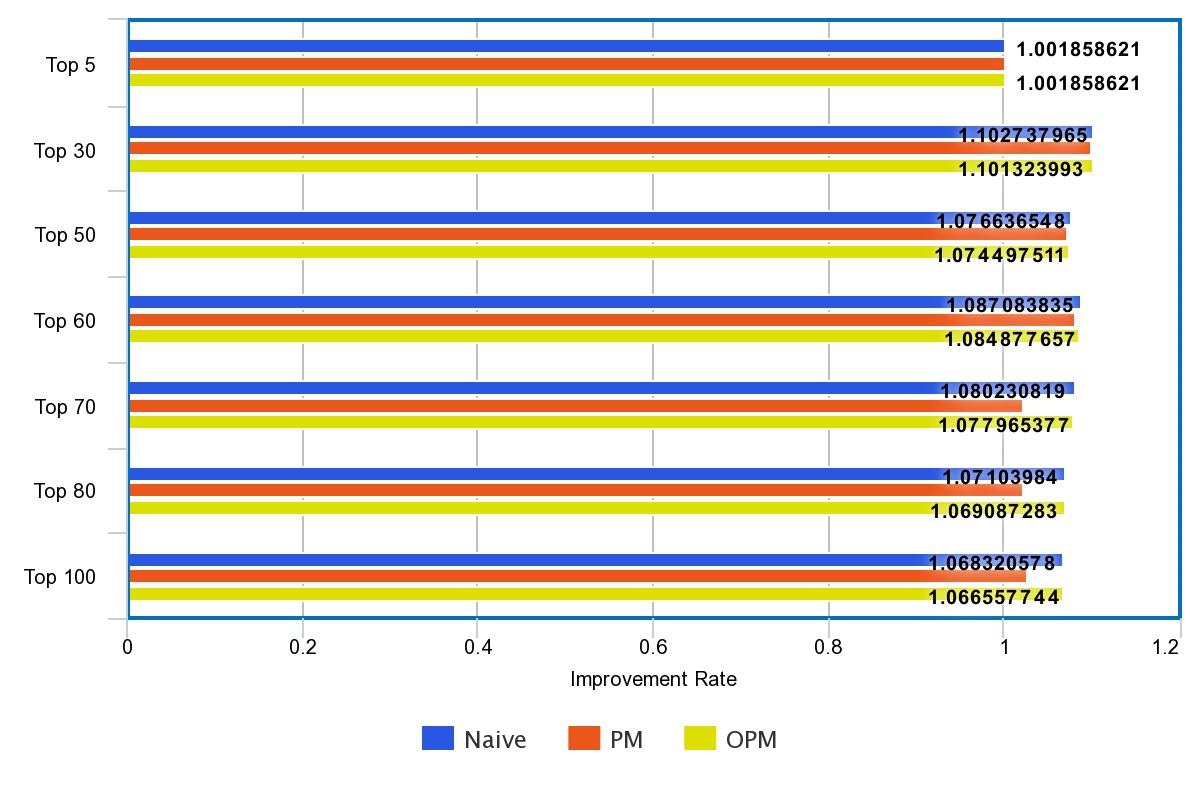
\includegraphics[width=0.85\textwidth]{figures/table_1_5_wikidata.jpeg}
\caption{The Average Conviction Improvement Rate (\%) of Rules Revised using Our Methods and Wikidata Football Dataset.}
\label{fig_1_5_wikidata}
\end{figure}

\section{Prediction Quality}

We now describe the evaluation procedure for estimating the predictive quality of the revised rules. Among top-50 (for IMDB, YAGO3) and top-300 (for Wikidata Football) positive rules mined from the KG, 5 are sampled as $\cR_H$ and then the revision procedure is applied for these rules. After that, the predictions of the rules from $\cR_H$ and their revisions are analyzed to evaluate our approaches.

To this end, these rulesets are applied to the learning KG $\cG^a$ and the corresponding predicted facts are generated by DLV tool~\cite{dlv}. Subsequently, we achieve $\cG_{\cR_\mi{H}}$, $\cG_{\cR_\mi{N}}$, $\cG_{\cR_\mi{PM}}$ and $\cG_{\cR_\mi{OPM}}$ for $\cR_H$ and revisions of $\cR_H$, resp. The statistics is shown in Table~\ref{tab:prediction_res}, where the first three columns indicate the head relations of the rules in $\cR_H$, the number of new predictions, i.e. predicted facts not included in $\cG^a$ and the part of these predictions which are outside $\cG^i_{\mi{appr}}$, resp. The statistics in the second and third columns is available for positive rules and all of their revisions.

\begin{table}[ht]
\centering

% \begin{tabular}{c|l|llll|llll}
% \hline
%  \multirow{2}{*}{}              &   \multirow{2}{*}{\textbf{$\mi{head(r)}$}}   	& \multicolumn{4}{c|}{\textbf{predictions}} 						&  \multicolumn{4}{c}{\textbf{outside $\cG^i_{appr}$}}  				\\ \cline{3-10} 
%          						&  									& $\cR_\mi{H}$  & $\cR_{N}$ & $\cR_{PM}$  		& $\cR_{OPM}$ &  $\cR_\mi{H}$     & $\cR_{\mi{N}}$ 	& $\cR_\mi{PM}$     & $\cR_{\mi{OPM}}$    \\ \hline
% %\multirow{4}{*}{\rotatebox{90}{YAGO}}
% & directed & 41079 & 39174 & 39174 & 39174  & 41021 & 39116 & 39116 & 39116 \\ %\cline{2-10}
%  & gradFrom & 3519 & 3456 & 3456 & 3456  & 3363 & 3300 & 3300 & 3300 \\ %\cline{2-10}
%  & citizenOf & 3407 & 2883 & 2883 & 2883  & 3360 & 2836 & 2836 & 2836 \\ %\cline{2-10}
%  & bornIn & 110283 & 108317 & 109846 & 108317 & 109572 & 107607 & 109137 & 107607 \\ \hline\hline %\cline{1-10}
% %\multirow{4}{*}{\rotatebox{90}{IMDB}} 
% & actIn & 1231 & 1214 & 1230 & 1214 & 1148 & 1131 & 1147 & 1131 \\ %\cline{2-10}
%  & genre & 629 & 609 & 618 & 609  & 493 & 477 & 482 & 477 \\% \cline{2-10}
%  & hasLang & 173 & 102 & 125 & 102 & 163 & 92 & 115 & 92 \\ %\cline{2-10}
%  & prodIn & 2489 & 2256 & 2327 & 2327 & 2488 & 2255 & 2326 & 2326 \\ \cline{1-10}
% \end{tabular}
\footnotesize{
\resizebox{\columnwidth}{!}}}  				\\ \cline{2-12} 
 		& $\cR_\mi{H}$  & $\cR_{\mi{N}}$ & $\cR_{\mi{PM}}$  		& $\cR_{\mi{OPM}}$ &  $\cR_\mi{H}$     & $\cR_{\mi{N}}$ 	& $\cR_\mi{PM}$     & $\cR_{\mi{OPM}}$  & $\cR_{\mi{N}}$ 	& $\cR_\mi{PM}$     & $\cR_{\mi{OPM}}$   \\ \hline

%\multirow{4}{*}{\rotatebox{90}{IMDB}} 
 $\mi{{I}{:}{actedIn}}$ & 1231 & 1214 & 1230 & 1214 & 1148 & 1131 & 1147 & 1131 &90 & 100 & 90\\ %\cline{2-10}
 $\mi{{I}{:}{genre}}$ & 629 & 609 & 618 & 609  & 493 & 477 & 482 & 477 &50 & 20 & 50\\% \cline{2-10}
 $\mi{{I}{:}{hasLang}}$ & 173 & 102 & 125 & 102 & 163 & 92 & 115 & 92 &  60 & 100 & 60\\ %\cline{2-10}
 $\mi{{I}{:}{prodIn}}$ & 2489 & 2256 & 2327 & 2327 & 2488 & 2255 & 2326 & 2326 & 10 & 10 & 30 \\ \cline{10-12}
 &  &  &  &  &  &  &  &  	& 52.50  & 45.16   & \textbf{57.75}  \\
\hline 
$\mi{{Y}{:}{direct}}$ & 41079 & 39174 & 39174 & 39174  & 41021 & 39116 & 39116 & 39116 & 100 & 100 & 100   \\
 $\mi{{Y}{:}{grFrom}}$ & 3519 & 3456 & 3456 & 3456  & 3363 & 3300 & 3300 & 3300 & 100 & 100 & 70 \\ 
 $\mi{{Y}{:}{citizOf}}$ & 3407 & 2883 & 2883 & 2883  & 3360 & 2836 & 2836 & 2836 & 50 & 50 & 70 \\ 
 $\mi{{Y}{:}{bornIn}}$ & 110283 & 108317 & 109846 & 108317 & 109572 & 107607 & 109137 & 107607 &90& 90 & 100 \\ \cline{10-12}  
 &  &  &  &  &  &  &  &  	& 85  & 85   & 85 \\
 \hline 
 \end{tabular}}}

\smallskip
\caption{New Facts Predicted by the Rulesets for IMDB (\textit{I}), YAGO (\textit{Y}) and Wikidata Football (\textit{W}).}
\label{tab:prediction_res}
%\vspace*{-1.7\baselineskip}
\end{table}

One can see that not many predicted facts are included in $\cG^i_{\mi{appr}}$ ($\approx$9\% for IMDB and $\approx$2\% for YAGO ideal KGs). This can be explained by the fact that YAGO is a highly incomplete general purpose KG. Moreover, it is crucial to note that the sampled Horn rules and their revisions generate approximately the same number of correctly predicted facts which are present in $\cG^i_{\mi{appr}}$. More specifically, in all three datasets $\cG_{\mi{\cR_H}}\backslash \cG_{\mi{\cR_{PM}}} \cap \cG^i_{\mi{appr}}=\emptyset$ means that the grey region has nothing in common with the approximated ideal KG in Figure~\ref{fig:venn}, in other words, the addition of exceptions does not lead to the removal of correct predictions from $\cG^i_{\mi{appr}}$.

To guarantee the fairness of the comparison between predictions generated by different rulesets, it is necessary to keep the $\cR_H$ not totally incorrect. Indeed, provided that the sampled positive rules always generate inaccurate facts, inserting arbitrary negated atoms may filter out some incorrect predictions, resulting in the rule enhancement, yet the rules themselves would still be of poor quality. Furthermore, observe that the number of predictions made by $\cR_H$ outside $\cG^i_{\mi{appr}}$ (third column of Table~\ref{tab:prediction_res}) is rather large. To verify these predictions, unfortunately no ground truth is available. Thus, we have to manually check the generated facts using the Internet resource. Since the number of the facts to be checked is huge, we propose to randomly select maximum 20 new predictions for each head predicate in $\cR_H$ and verify them. For the IMDB, YAGO and Wikidata Football, 70\%, 30\% and 55\% of predictions respectively turned out to be indeed correct. This shows that the quality of the positive rules that we start with is acceptable.

Since the size of the set difference between predictions made by $\cR_H$ and extended by applying $\cR_H$ and its revisions is also huge, we have to proceed further with sampling to evaluate the predictive quality of the revision. Here for each head relation from the set differences $\cG_{\cR_\mi{H}}\backslash \cG_{\cR_{\mi{N}}}$, $\cG_{\cR_\mi{H}}\backslash \cG_{\cR_{\mi{PM}}}$ and $\cG_{\cR_\mi{H}}\backslash \cG_{\cR_{\mi{OPM}}}$, 10 facts have been randomly sampled for manual check. In the last column of the Table~\ref{tab:prediction_res}, the proportion of incorrect facts in the difference sets are presented. These facts are called ``correctly removed", since they correspond to false prediction made by $\cR_H$ but avoided by the respective revisions (the grey region in in Figure~\ref{fig:venn}). For the IMDB dataset, among all the revision strategies, OPM ranking always performs best with 57.75\% and 97.5\% correctly removed predictions for IMDB and Wikidata Football, resp. Meanwhile, all the rankers demonstrate the same results (85\%) for the YAGO KG. Since the predictive power of the positive rules in IMDB is better than those in YAGO, the revision of the latter makes a more visible impact than the former.

\section{Running Times}

In our experiment, top-100 positive rules are mined from IMDB and YAGO while this number of Wikidata Football is 300. Table~\ref{tab:run_time} provides statistics about running times (in seconds) of three different steps in the RUMIS system. More specifically, the second row of this table indicates how long for mining Horn rules and exception witness sets. In addition, the third and fourth rows present the average running times (over three ranking methods Naive, PM, OPM) of resp. ranking exceptions and extending KGs with DLV.

\begin{table}[ht]
\centering
\footnotesize{
\begin{tabular}{|c|ccc|}
\hline
\textbf{Steps} & \textbf{IMDB} & \textbf{YAGO} & \textbf{Wikidata Football}\\
\hline
 \textit{Horn Rule and EWS Mining} & 7 & 68 & 193\\
 \textit{Exception Ranking} & 32 & 111 & 2940\\
 \textit{Extension with DLV} & 8 & 310 & 180\\
 \hline 
\end{tabular}
}
\smallskip
\caption{Running Times for Each Step of the Three Datasets}
\label{tab:run_time}
%\vspace*{-1.7\baselineskip}
\end{table}

It can be seen that the numbers of Wikidata Football for the first two steps are the largest since the quantity of positive rules mined from this dataset is much bigger than that of IMDB or YAGO. Meanwhile, among the three datasets, YAGO has the most number of facts, resulting in the longest time to extend the KG using DLV (310 seconds).

\begin{figure}[t]
    \centering
   
    \vspace{-.2cm}
    \begin{tabular}{l}
 {\scriptsize
        $\mi{r_1: writtenBy(X, Z)}  \leftarrow
        \mi{hasPredecessor(X, Y)},\mi{writtenBy(Y, Z)},$ $ \textbf{not}$  $\mi{american\_film(X)} $}\\        
       {\scriptsize 
$\mi{r_2:  actedIn(X, Z)}  \leftarrow
        \mi{isMarriedTo(X, Y)},\mi{directed(Y, Z)},$ $ \textbf{not}$  $\mi{silent\_film\_actor(X)} $} \\
          {\scriptsize 
$\mi{r_3:  isPoliticianOf(X, Z)}  \leftarrow
        \mi{hasChild(X, Y)}{,}\mi{isPoliticianOf(Y, Z)}{,}$$ \textbf{not}$  $\mi{vicepresidentOfMexico(X)} $} \\
 \end{tabular}            
    \caption{Examples of the Revised Rules}
 \label{fig:examplerules}
 \vspace{-.4cm}
\end{figure}

\textbf{Example rules.} Some interesting examples are presented in the Figure~\ref{fig:examplerules}. Here 
the rule $\mi{r_1}$ mined from IMDB dataset indicates that normally movies in the same series are written by the same writer except the American movies. The rule $\mi{r_3}$ generated from YAGO reveals an interesting pattern from domain politics, i.e, typically fathers and sons are politicians in the same country unless the fathers are Mexican vice-presidents.

\chapter{Conclusions and Future Work}
\label{chap:conclusion}

In this research work, we develop the RUMIS system based on the theory framework where the novel concept of \textit{partial materialization} is introduced to revise positive Horn rules. Subsequently, the chosen revisions are exploited to extend the original data, and thus, tackle the KG completion problem. Besides, some experiments are conducted for testing quality of rules generated by RUMIS and the result supports the proposed theory. In the future, there are some directions that we can develop as follows.

\begin{itemize}
\item More forms for the positive rules can be implemented, not only the form~\ref{form2} introduced in Chapter~\ref{chap:back}. This makes the RUMIS less restrictive and diversify the resulting revisions.
\item Due to large size of the KG, data indexing is a time burden step for every experiment. Thus, we can refine the RUMIS system by store the indices in a database and the rest computation may make us that via a web service subsequently.
\item Other predictive measures and exception evaluation methods can be tested to search for interesting nonmonotonic rules.
\end{itemize}


% *************** Bibliography ***************
\bibliographystyle{plain}
{\small\bibliography{bibliography/reference}}
\clearpage

% *************** Appendixes ***************
\addtocontents{toc}{\vspace{2em}}
\appendix
%\appendixpage*


% *************** Back matter ***************
%\backmatter
%\input{back.tex}

\end{document}